Molecular modeling seeks to gain new insights into the real world behavior of molecules by mimicking these molecules, usually using computer simulations.
According to the theory of ``minimal frustration'' the protein native state is not only a low energy state, but is also stable \cite{bryngelson1987spin}.
So the prediction of native or native-like conformations focuses on finding those conformations which have a low potential energy.
As measuring the true potential energy of a system is very difficult or impossible computational models seek to reproduce the qualitative behavior of the energy surface.
Quantum mechanics calculations are often viewed as the gold standard with respect to intramolecular energy calculations.
However, despite the accuracy of quantum mechanics, its application to large systems such as proteins is currently limited due to the amount of time necessary to perform quantum mechanics calculations on a large number of atoms.
Instead quantum mechanics calculations have been used to parameterize a majority of the most popular molecular mechanics force fields currently in use, including:
\begin{enumerate}
\item AMBER \cite{weiner1984new},
\item OPLS-AA \cite{kaminski1994free},
\item and CHARMM \cite{mackerell2002charmm}.
\end{enumerate}

The earliest molecular mechanics force fields either modeled groups of atoms as a unit, hydrogens being grouped with their bound heavy atom \cite{jorgensen1988opls}, or even each residue as a unit \cite{lee1999energy}, both to reduce the number of parameters in the model and to increase the speed of computations.
Although {\it ab initio} folding experiments are theoretically interesting, they are generally not practical both because of the difficulty in simulating such a large system for the time-frame necessary to observe behaviors like folding, and also because structural models for many proteins are available either directly as X-ray structures, or indirectly through homology.

\begin{figure}[h]
\begin{center}
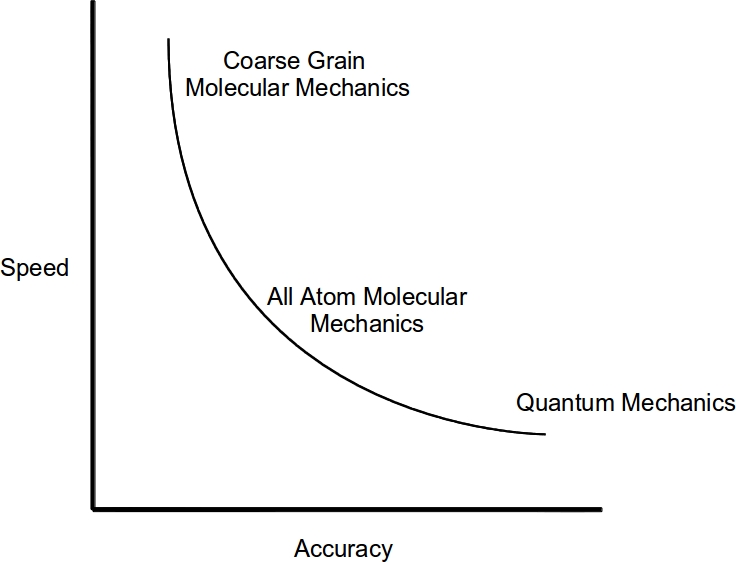
\includegraphics[width=0.7\textwidth]{figures/conservation_of_annoyance.png}
\caption{To an extent it is always possible to either increase accuracy or decrease running time, or the cost of an experiment.
New scientific methods should allow one to increase accuracy while not spending additional time.}
\label{figure:conservation_of_annoyance}
\end{center}
\end{figure}

Because of the evolutionary cost of mis-folded proteins, proteins have been selected to minimize mis-folding, making the general shape of the potential energy surface roughly funnel shaped with the native structure at the minimum \cite{leopold1992protein}.
Despite this shape, the energy landscape of proteins is a very ``jagged'' surface with a large number of local minima \cite{tsai1999folding}.

Even the smallest enzyme contains 62 amino acids, and has thousands of degrees of freedom \cite{chen19924}, and larger enzymes are regularly more than 1000 amino acids.
The number of degrees of freedom of these systems make any attempt to analytically solve for a global minimum energy conformation impossible, and require other methods of generating plausible conformations.
In order to compensate for this a number of different sampling methods have been developed.

%\subsection{Sampling Methods}
%\label{subsection:sampling_methods}

%    \subsubsection{Minimization}
%    \label{subsubsection:minimization}
%    Minimization techniques seek to find the lowest energy conformation in a given potential well.
Generally, they make no attempt to sample outside of that well, and therefore are frequently implemented as a final stage in sampling, in order to relieve any unfavorable interactions in proposed structures.
There are a large number of different minimization techniques, and they will not be covered in any real depth here, please see the original papers for more details, or \cite{schlick2010molecular} for a review.
As the basic terms of the general molecular mechanics potential energy function are differentiable, and discounting for the moment the significant effects of solvent, it is possible to solve for the energy gradient, or force on every atom for a given conformation.
A few minimizations methods include:
\begin{enumerate}
\item ``Steepest descent'', conceptually the simplest minimization algorithm, in which the gradient is calculated at each step, and the size of the step is proportional to the magnitude of the gradient \cite{levitt1969refinement,bixon1967potential}.
\item ``Newton'' methods instead of approximating the gradient as a linear function in a small neighborhood, express the gradient, as a quadratic function.  This has been shown to converge more quickly than steepest descent \cite{ponder1987efficient}.  
Discrete Newton and Quasi-Newton methods use numeric estimation techniques instead of analytically solving for the gradient \cite{schlick2010molecular}.
\item ``Truncated Newton'' methods find an approximate solution to Newton's equations, forcing the residual to approach zero as the series converges \cite{dembo1983truncated}. 
\end{enumerate}

% molecular mechanics burkert allinger

%Quasi-Newton methods like ABNR of CHARMM estimate the hessian, instead of computing it directly, by accumulating residuals over multiple steps \cite{chu2003super}.


%    \subsubsection{Monte-Carlo Sampling}
%    \label{subsubsection:monte_carlo}
%    Metropolis Monte-Carlo simulation was originally developed in the 1950's to provide rapid sampling of the solution space of many variable problems \cite{metropolis1953equation,hastings1970monte}.
Monte-Carlo techniques generate a sequence of states from a distribution by proposing a new state based only on the current state 
If the ensemble average is the same as the sequence average, a Monte Carlo Markov chain can be used to estimate ensemble averages, this is known as {\it ergodicicy} \cite{schlick2010molecular}.
Another requirement is {\it detailed balance} that the probability of transition from a state $X_{i}$ to a state $X_{i+1}$ is the same as the probability of the reverse transition, i.e. $X_{i+1}$ to $X_{i}$.
By setting the probability of acceptance to
\begin{equation}
\label{equation:metropolis_acceptance}
P(x \rightarrow x') = min\left(1,e^{-\frac{{\Delta}E}{k_{B}T}}\right)
\end{equation}

these conditions are met.

In molecular mechanics, Metropolis Monte Carlo provides a very efficient means of sampling conformation space and a simple method of estimating the distribution of states.
Modifications on this method, such as annealing, where the temperature is continuously decreased over the course of the simulation, or umbrella sampling, which attempts to achieve better sampling in cases where a potential energy barrier divides two or more states from each other \cite{torrie1977nonphysical}.
While Monte Carlo sampling techniques are very fast to provide new states, the majority of these states reflect higher energy conformations.
Since it is of practical biological interest, Monte Carlo minimization has been developed to increase the rate at which minima are sampled \cite{li1987monte}.



%    \subsubsection{Analytic Loop Closure}
%    \label{subsubsection:analytic_loop_closure}
%    Subsequences with regular secondary structures, i.e. $\alpha$-helices and $\beta$-sheets are generally better conserved, and therefore likely to be well covered by simple homology models \cite{kolodny2005inverse,petrey2003using}.
The intervening ``random coil'' or loop regions often play a large role in determining protein specificity for a specific ligand, as in antigen-antibody binding \cite{bajorath1996comparison}, small protein toxins to the receptors they target \cite{wu1996functional}, or transcription factors to specific DNA sequences \cite{jones1999protein}.

Loop closure or prediction is a significant part of homology modeling \cite{petrey2003using} and building structures consistent with X-ray refraction data.
Therefore, in order to accurately predict three dimensional structure through homology models, infer protein binding partners and function, or even build a three dimensional structure consistent with both X-ray data and physical constraints, accurately predicting these loop regions is critical \cite{fiser2000modeling}.

The loop closure question is, given two fixed endpoints and a flexible loop, or actuator, how does one find a loop conformation, or set of conformations, that connects the two endpoints.
Because similar problems are frequently encountered in the field of robotics, a number of loop closure algorithms have been adapted from robotics \cite{kolodny2005inverse}.
The first of these algorithms is analytical loop closure, where a conformation that satisfies the closure criteria is solved for directly by solving a system of equations.
Though this problem can be solved analytically for small loops \cite{wedemeyer1999exact,go1970ring,bruccoleri1985chain,palmer1991standard}, the difficulty of the problem increases as loop length grows and the number of degrees of freedom of the loop section increases.
Additionally, these closure constraints make sampling multiple different conformations more difficult \cite{cortes2005sampling}, though it is possible to hierarchically solve sub-loops in order to generate conformations for possible complete loop conformations \cite{wedemeyer1999exact}.


%    \subsubsection{Random Tweak}
%    \label{subsubsection:tweak}
%    Random tweak, like CCD, is a method of producing and sampling closed loop conformations.
It begins in much the same way as CCD, by randomizing $\phi$ and $\psi$ dihedral angles of the loop backbone.
Random tweak seeks to close the loop while retaining dihedral angles as close to the randomized starting structure as possible.
By adjusting each dihedral only a small amount at a time and staying in the region where $sin(\theta) \approx \theta$, it is possible to formulate a set of linear equations to solve for a set of $\Delta\theta_{i}$, which minimizes the distance between the crystal position of the atom to be closed and the random position.
Because the assumption $sin(\theta) \approx \theta$ only holds for small $\theta$, the maximum change in angle is limited to 10 degrees in the original implementation of the random tweak algorithm.
Because almost all structures predicted using the random tweak or cyclic coordinate descent produce closed loops, a much smaller fraction of time is spent sampling loops that do not satisfy the closure criteria, making these algorithms very efficient \cite{fine1986predicting,shenkin1987predicting}.


%    \subsubsection{Cyclic Coordinate Descent}
%    \label{subsubsection:cyclic_coordinate_descent}
%    Another robotics algorithm which has been successfully applied to protein loop closure is Cyclic Coordinate Descent (CCD) \cite{canutescu2003cyclic}.
As the length of a flexible loop grows the number of degrees of freedom increases and the possible solution space grows exponentially. 
Cyclic coordinate descent seeks to close the loop by adjusting the degrees of freedom, in this case the $\phi$ and $\psi$ dihedral angles, sequentially and possibly iterating over each degree of freedom multiple times until the loop is closed.
This method is able to solve for conformations very quickly, and the likelyhood of closing a loop {\it increases} as the number of degrees of freedom of the system increases.

In cyclic coordinate descent the $\phi$ and $\psi$ angles of each loop backbone residue are first randomized.
Then a loop dihedral is chosen at random, and varied to move the last atom of the loop as near as possible to its desired position.
A new dihedral is chosen and optimized until the loop is closed.
It is possible that this procedure does not converge to a closed state, however experiments have shown that this is very unlikely even for extended loops with few degrees of freedom, $ < 2\%$ failure rate for 4 residue loops.
Solving for the ideal dihedral angle at each step is a simple optimization problem making CCD a very fast algorithm \cite{wang1991combined,canutescu2003cyclic}.
In experiments CCD produces closed loop candidates in ~1/6 the time of the random tweak method.

A variation on cyclic coordinate descent seeks to close the loop by not only requiring atom closure, but by requiring that the entire backbone of the closure residue is superimposed, within some geometric similarity tolerance, between the predicted and crystal structure.
This constrainint ensures that the angles and dihedrals of the closure residue are reasonable\cite{canutescu2003cyclic}.


%    \subsubsection{Rotamer Assembly}
%    \label{subsubsection:rotamer_assembly}
%    Rotamer assembly or systematic search shares some similarity with fragment buildup techniques in that it uses a rotamer library to assemble possible loops.
This rotamer library represents the common backbone dihedrals for each amino acid.
This method operates by dividing the loop into two pieces, usually in half, and considering all possible half loops which can be built using rotamer library \cite{moult1986algorithm}.
For each side of the loop a ``tree'' is considered in both a physical sense, that the hemi-loop branches as it grows away from its anchor, and a decision tree sense, in that every residue represents a decision where a single rotamer is selected from the rotamer library.
When the hemi-trees for each side of the gap are fully constructed some closure criteria is applied, in the case of the original systematic search geometric agreement is required of the entire mid-residue \cite{moult1986algorithm}, however a more lax criteria is applied in the case of the PLOP where only one atom is required to be approximately superimposed \cite{jacobson2004hierarchical}.
By carefully pruning trees during the building process, and biasing the search towards occupied regions of $\phi$-$\psi$ space, systematic search can be quite efficient, spending little time sampling implausible regions of conformation space.
Additionaly, by building residue pairs, using a smaller
 possibly restricting the rotamer library by building multiple residues at a time this sort of procedure has been used to build loops of 20+ residues \cite{zhao2011progress}.


% \cite{kolodny2005inverse}


\subsection{Energy Functions}
\label{subsection:energy_functions}
    \subsubsection{The General Form of the Energy Model}
    \label{subsubsection:energy_general_form}
    Some energy models do not seek to accurately rank potential conformations, fast ``screening'' functions attempt to quickly differentiate physically impossible conformations from plausible conformations without performing an expensive minimization or energy calculation step.
Application of these screening functions has the potential to greatly reduce the number of potential conformations that must be scored using the full detail energy function, greatly decreasing the overall cost of conformation prediction.
These screening criteria can be applied either during the sampling procedure, potentially eliminating sampling of a large area of excluded conformation space, or after sampling before a more expensive energy function is applied to rank conformations.
Effective screening criteria have a large impact on the total performance of a structure prediction method.

One of the earliest screening criteria was the hard sphere overlap collision detection \cite{levinthal1966molecular}, and this method is consistently included in screening scriteria.
Other screens include:
\begin{enumerate}
\item bounds on bond lengths and angles, as a single bond which deviates significantly from equilibrium can dominate the energy of a conformation,
\item limitations on $\phi$-$\psi$ space occuped by backbone dihedrals corresponding to the Ramachandran plot of the residue,
\item limiting side chain dihedrals to staggered conformations, which correspond to the low energy well of side chain dihedral space \cite{moult1986algorithm},
\item excluding structuctures which present excessive solvent accessible surface area, as this conflicts with the hydrophobic effect, which has a large effect on the conformation of the native state \cite{chothia1975principles}
\item limitations on the number of ``dry'' cavities, and the number of internal charged residues \cite{moult1986algorithm}
\end{enumerate}

The general form of most molecular mechanics energy potentials is reasonably consistent, with bonds and angles being modeled as a spring, dihedrals as a Fourier series.
\begin{equation}
E \left(r^N \right ) = E_\mathrm{bonds} + E_\mathrm{angles} + E_\mathrm{dihedrals} + E_\mathrm{nonbonded}
\label{equation:opls}
\end{equation}

\begin{equation}
E_\mathrm{bonds} = \sum_\mathrm{bonds} K_r (r-r_0)^2
\end{equation}

\begin{equation}
E_\mathrm{angles} = \sum_\mathrm{angles} k_\theta (\theta-\theta_0)^2
\end{equation}

\begin{equation}
E_\mathrm{dihedrals} = \sum_{i=1\dots4} {\frac {V_i} {2} \left [ 1 + \cos \left ( i * (\phi-\phi_0) \right ) \right ] }
\end{equation}

The non-bonded terms are modeled as a Columbic potential between any point charges and a Lennard-Jones or 6-12 potential between any non-bonded atoms.
These non-bonded atoms are phased in by a ``fudge factor'' for atoms in a 1-4 configuration.
\begin{equation}
\begin{split}
E_\mathrm{nonbonded} = \sum_{i>j} f_{ij} 
                \left (
                        \frac {q_i q_j e^2}{r_{ij}}
                    + 4 \epsilon_{ij} 
                    \left  [  
                        \left ( \frac{\sigma_{ij}}{r_{ij}}\right )^{12}
                      - \left ( \frac{\sigma_{ij}}{r_{ij}}\right )^{6}
                    \right ]
                \right )
\\
f_{ij} = 
  \begin{dcases*}
   0    & if $i$ and $j$ are separated by 2 or fewer bonds\\
   0.5  & if $i$ and $j$ are separated by 3 bonds\\
   1.0  & otherwise
  \end{dcases*}
\end{split}
\end{equation}

Where $\sigma_{ij} = \sqrt{\sigma_{ii} \sigma_{jj}}$ and $\epsilon_{ij} = \sqrt{\epsilon_{ii}\epsilon_{jj}}$ \cite{jorgensen1996development}.



    \subsubsection{Molecular Surfaces}
    \label{subsubsection:molecular_surfaces}
    Central to the discussion of solvent is a discussion of how to formulate the surface of a protein.
The most frequently used formulations of surface area include:
\begin{enumerate}
\item The Van der Waals (VDW) surface is the surface formed by the VDW radius of each molecule, though sometimes differing parameters are used for the VDW radii, and the ideal radii may even vary by application.
\item The solvent accessible surface, which is defined as the surface traced by the center of a spherical probe ``rolled'' over the VDW surface \cite{richards1977areas}.  This idea is very closely related to the idea of the solvent excluded volume, or the shape of the solvent cavity enforced by the VDW surface of the molecule \cite{richmond1984solvent}.
\item The molecular surface, or Connolly surface, is composed of the VDW surface in areas where the spherical probe touches the VDW surface, in union with all points on the probe ``between'' two points on the VDW surface when the probe is contacting multiple atoms \cite{connolly1983analytical}, put another way the surface of the volume which intersects no possible probe location.
\end{enumerate}
Frequently these surfaces are approximated numerically, using the Shrake-Rupley algorithm \cite{shrake1973environment}, by considering a spherical mesh about every atom and including only points which satisfy the definition of the surface, or using these points to interpolate a surface.

The significance of surface area is determined by physical constraints but can be well illustrated by a number of observations about proteins.
First the ratio of total area of a theoretical unfolded, i.e. linearly arranged, protein to its length is almost among proteins, only varying by \textapprox 3\% between different proteins.


\subsection{Solvent Models}
\label{subsubsection:solvent_models}
The section on solvent models.

